\begin{frame}
    \frametitle{Обробка слайдів}
    Складність швидкої медіани $m$ зображень, кожне з яких розміром $h \times w$:
    $\mathcal{O}(h \cdot w).$ \\
    Для звичайної часової медіани із quick sort: $\mathcal{O}(h \cdot w \cdot m^2)$ у найгіршому випадку. \\
    Варто відмітити, що таке прискорення досягається тим,
    що є обмеження на використання значень від $0$ до $255$.
    \begin{figure}[H]
        \centering
        \subfloat[До швидкої медіани]{
            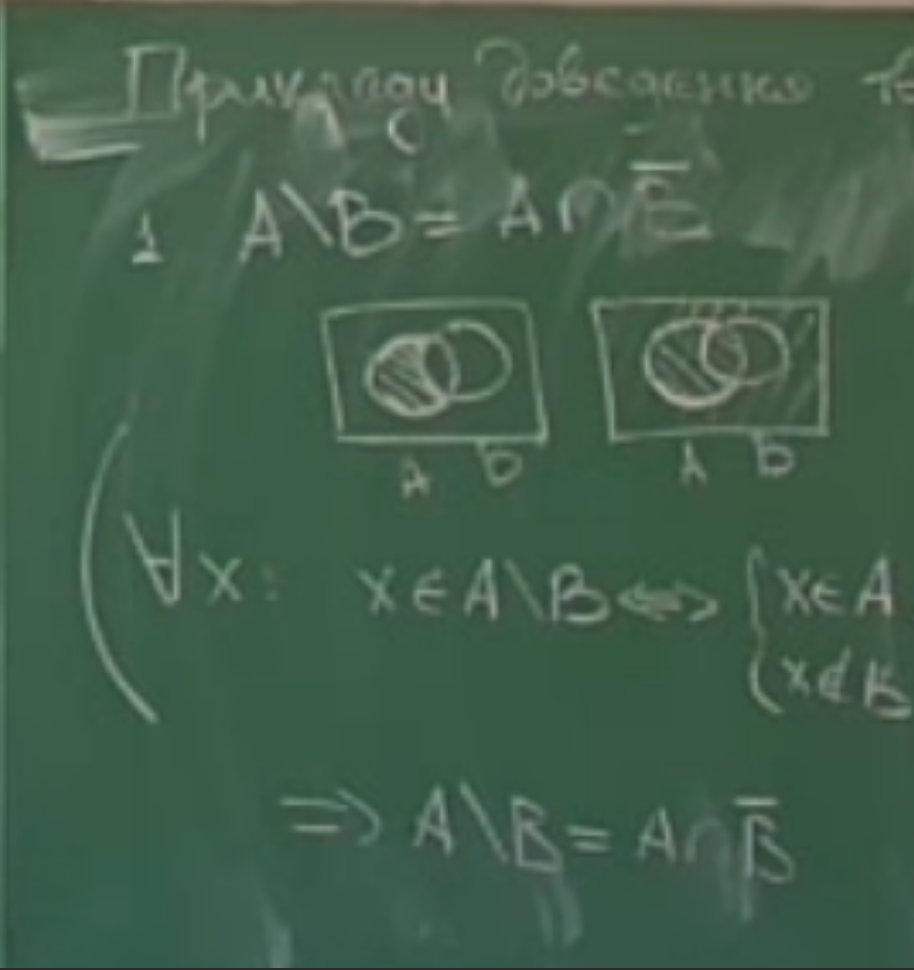
\includegraphics[width=0.35\textwidth]{images/frame_before_median}
        }
        \subfloat[Після швидкої медіани]{
            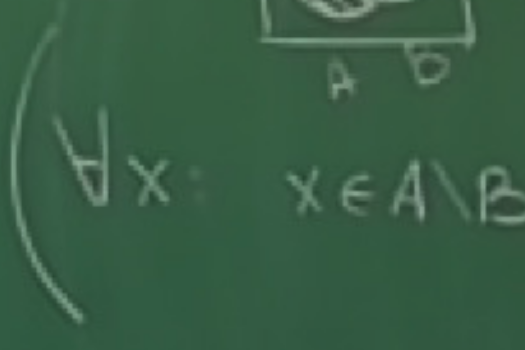
\includegraphics[width=0.35\textwidth]{images/frame_after_median}
        }
        \caption{Джерело ~---~\url{https://youtu.be/a7TUp4p-pIk}
        }
    \end{figure}
\end{frame}
